\documentclass[11pt]{article}
% Packages
\usepackage[T1]{fontenc} % Fontes T1
\usepackage[utf8]{inputenc} % Input UTF8
\usepackage{csquotes}
\usepackage[portuguese]{babel} %Usar língua portuguesa
\usepackage{blindtext}
\usepackage{graphicx}
\usepackage{geometry}
\usepackage{float}
\usepackage{hyperref}
\usepackage{indentfirst}
\usepackage[printonlyused]{acronym}
\usepackage{ragged2e}
\usepackage{textcomp}
\usepackage{multicol}
\usepackage{listings}
\usepackage{color}
\usepackage{fancyhdr}
\usepackage{soul}


\geometry{a4paper,inner=20mm,outer=20mm,top=15mm, bottom=15mm}

% Define colors
\definecolor{dkgray}{rgb}{0.37,0.37,0.37}
\definecolor{gray}{rgb}{0.5,0.5,0.5}
\definecolor{mauve}{rgb}{0.58,0,0.82}
\definecolor{codegray}{RGB}{234, 234, 234}

\setlength{\parskip}{0.5em plus 0.1em minus 0.2em}
\setlength{\headheight}{134pt}

\fontsize{12}{12}\selectfont

\lstset{frame=tb,
  language=C,
  aboveskip=3mm,
  belowskip=3mm,
  showstringspaces=false,
  columns=flexible,
  basicstyle={\small\ttfamily},
  numbers=none,
  numberstyle=\tiny\color{gray},
  keywordstyle=\color{blue},
  commentstyle=\color{dkgray},
  stringstyle=\color{mauve},
  breaklines=true,
  breakatwhitespace=true,
  tabsize=4
}

\pagestyle{fancy}

% Header
\fancyhead[C]{
    \begin{center}
        
\includegraphics{images/ua}\\
        \vspace{2mm}
        \textbf{{\LARGE \title}}\\
        \vspace{2mm}
    \end{center}
}
\fancyhead[L]{\leftmark}
\fancyhead[R]{\thepage { -} \PreviousTotalPages}

% Document
\begin{document}

    % Define keybinds
    \def\title{\textbf{RELATÓRIO DE ANÁLISE DE COMPLEXIDADE}}
    \def\authorjp{João Bastos (113470)}
    \def\authorrg{Rúben Gomes (113435)}
    \def\authors{João Bastos (113470) e Rúben Gomes(113435)}
    \def\contacts{(113470) joaop.bastos@ua.pt, (113435) rlcg@ua.pt}
    \def\department{Departamento de Eletrónica, Telecomunicações e Informática}
    \def\university{Universidade de Aveiro}
    
    
\section{Introdução}\label{sec:introducao}

\fontsize{12}{12}\selectfont
    \par Na implementação do código image8bit.c, foram criadas diversas funções para manipular imagens
        de diferentes formas. Para além de implementar, é necessário analisá-las para garantir um 
        código mais eficiente. Para esse propósito, foram analisados os algoritmos das funções
        ImageLocateSubImage() e ImageBlur().

    \par O ficheiro image8bit.c contêm múltiplas funções para manipular imagens PGM(Portable Gray Map):

    \begin{itemize}
        \item \textbf{ImageValidPos} - Analisa se uma da posição corresponde a um píxel da imagem referida
            encontra-se fora da mesma
        \item \textbf{ImageValidRect} - Analisa se as dimensões correspondentes a um retângulo se encontram
            dentro da imagem ou não
        \item \textbf{ImageGetPixel e ImageSetPixel} - Responsáveis por obter o indíce do array de pixeis
            na respetiva posição e alterar esse valor por um outro.
        \item \textbf{ImageNegative} - Inverte os valores de cada pixel $(maxval - pixelValue)$
        \item \textbf{ImageThreshold} - Converte os valores de cada píxel para 0 ou para maxval
            se o mesmo for inferior ou superior ou igual respetivamente
        \item \textbf{ImageBrighten} - Converte os valores de cada píxel multiplicando por um fator
        \item \textbf{ImageRotate} - Cria uma imagem nova com os valores dos pixeis da original
            trocada de modo a obter uma imagem rodada 90º no sentido contrário dos ponteiros do relógio
        \item \textbf{ImageMirror} - Devolve uma imagem espelhada horizontalmente
        \item \textbf{ImageCrop} - Recorta uma parte da imagem e devolve-a noutra imagem
        \item \textbf{ImagePaste} - Insere uma imagem por cima de outra, certeficando que
            a imagem a inserir seja inferior à imagem onde será inserida
        \item \textbf{ImageBlend} - Junta 2 imagens, certifcando que a que se vai juntar seja 
         inferior à outra e é aplicado um valor $alpha$ entre 0.0 a 1.0
        \item \textbf{ImageMatchSubImage} - Compara se a partir de uma dada posição (x,y) 
            da imagem1 a imagem2 é igual
        \item \textbf{ImagemLocateSubImage} - Chama a função ImageMatchSubImage em cada píxel da
            imagem1 para comparar e define 2 ponteiros(px e py) para esse mesmo píxel
        \item \textbf{ImageBlur} - Aplica um filtro na imagem para criar uma desfocada
    \end{itemize}

    
    
    \newpage

    \section{ImageLocate}\label{sec:imagelocate}
\fontsize{12}{12}\selectfont
    \par A função ImageLocateSubImage() é usada para determinar se a imagem2 é uma parte da imagem1.
        Para esta função funcionar corretamente, esta chama a função ImageMatchSubImage() para comparar os pixeis 
        de modo a garantir que a imagem2 é, de facto, igual a uma parte da imagem1.

\subsection{Eficiência computacional da ImageLocateSubImage()}
    \par Para analisar a sua eficiência computacional, foi registado numa \autoref{tab:locate} o 
    número de comparações envolvendo uma sequência de testes com diferentes imagens. 

\begin{center}
    \begin{table}[h]
        \centering
        \begin{tabular}{| p{2cm} | p{3cm} | p{1.5cm} | p{2cm} | p{5cm} |}
        \hline
        \textbf{Img1} & \textbf{Img2} & \textbf{Iterações da Locate} & \textbf{Iterações da Match} & \textbf{Observações} \\ \hline
        original.pgm (300x300) & crop.pgm (100x100) & 3010 & 10000 & \\ \hline
        original.pgm (300x300) & rotate.pgm (300x300) & 90000 & 90000 & 
            img2 doesn't fit if it starts at another pixel other than (0,0) in img1 \\ \hline
        ireland.pgm (1600x1200) & airfield (1600x1200) & 1920000 & 1920000 &
            img2 doesn't fit in img1, if it starts in a different ixel than (0,0)  \\ \hline
        airfield (1600x1200) & ireland (640x480) & 1920000 & 1 &
            first pixel of img2 is different than img1, so the loop is only executed one time \\ \hline
        airfield (1600x1200) & airfieldCrop (100x100) & 1 & 10000 &  \\ \hline
        airfield (1600x1200) & airfieldCrop (10x10)  & 1 & 100 & \\ \hline
        airfield (1600x1200) & airfieldCrop (10x10) (no ponto 1549,1189) & 1903950 & 1898830 & \\ \hline                 
        \end{tabular}
        \caption{Tabela com dados resultantes das iterações da função ImageLocateSubImage() e ImageMatchSubImage()}
        \label{tab:locate}
    \end{table}
\end{center}

\newpage 

\par Com base na \autoref{tab:locate}, podemos afirmar sobre a sua comeplexidade:
\begin{itemize}
    \item \textbf{Best Case:} Imagens com pouca resolução e a imagem2 está localizada no pixel (0,0) $O(1)$
    \item \textbf{Average case:} Imagem tem pouca resolução e a imagem2 não se encontra localizada nela
    \item \textbf{Worst case:} Imagens com grande resolução e a imagem 2 não se encontra localizada $O(width * height)$
\end{itemize}

\subsection{Funcionamento da ImageLocateSubImage()}
    \par Este algoritmo segue uma lógica básica por detrás. Sâo enviadas duas imagens, img1 e img2, e é feita 
        a comparação entre os pixeis da img1 e da img2, sendo o ínicio no pixel (0,0) até ao pixel ($width,$height),
        tal como consta na \autoref{fig:locate}.

    \begin{figure} [H]
        \centering
        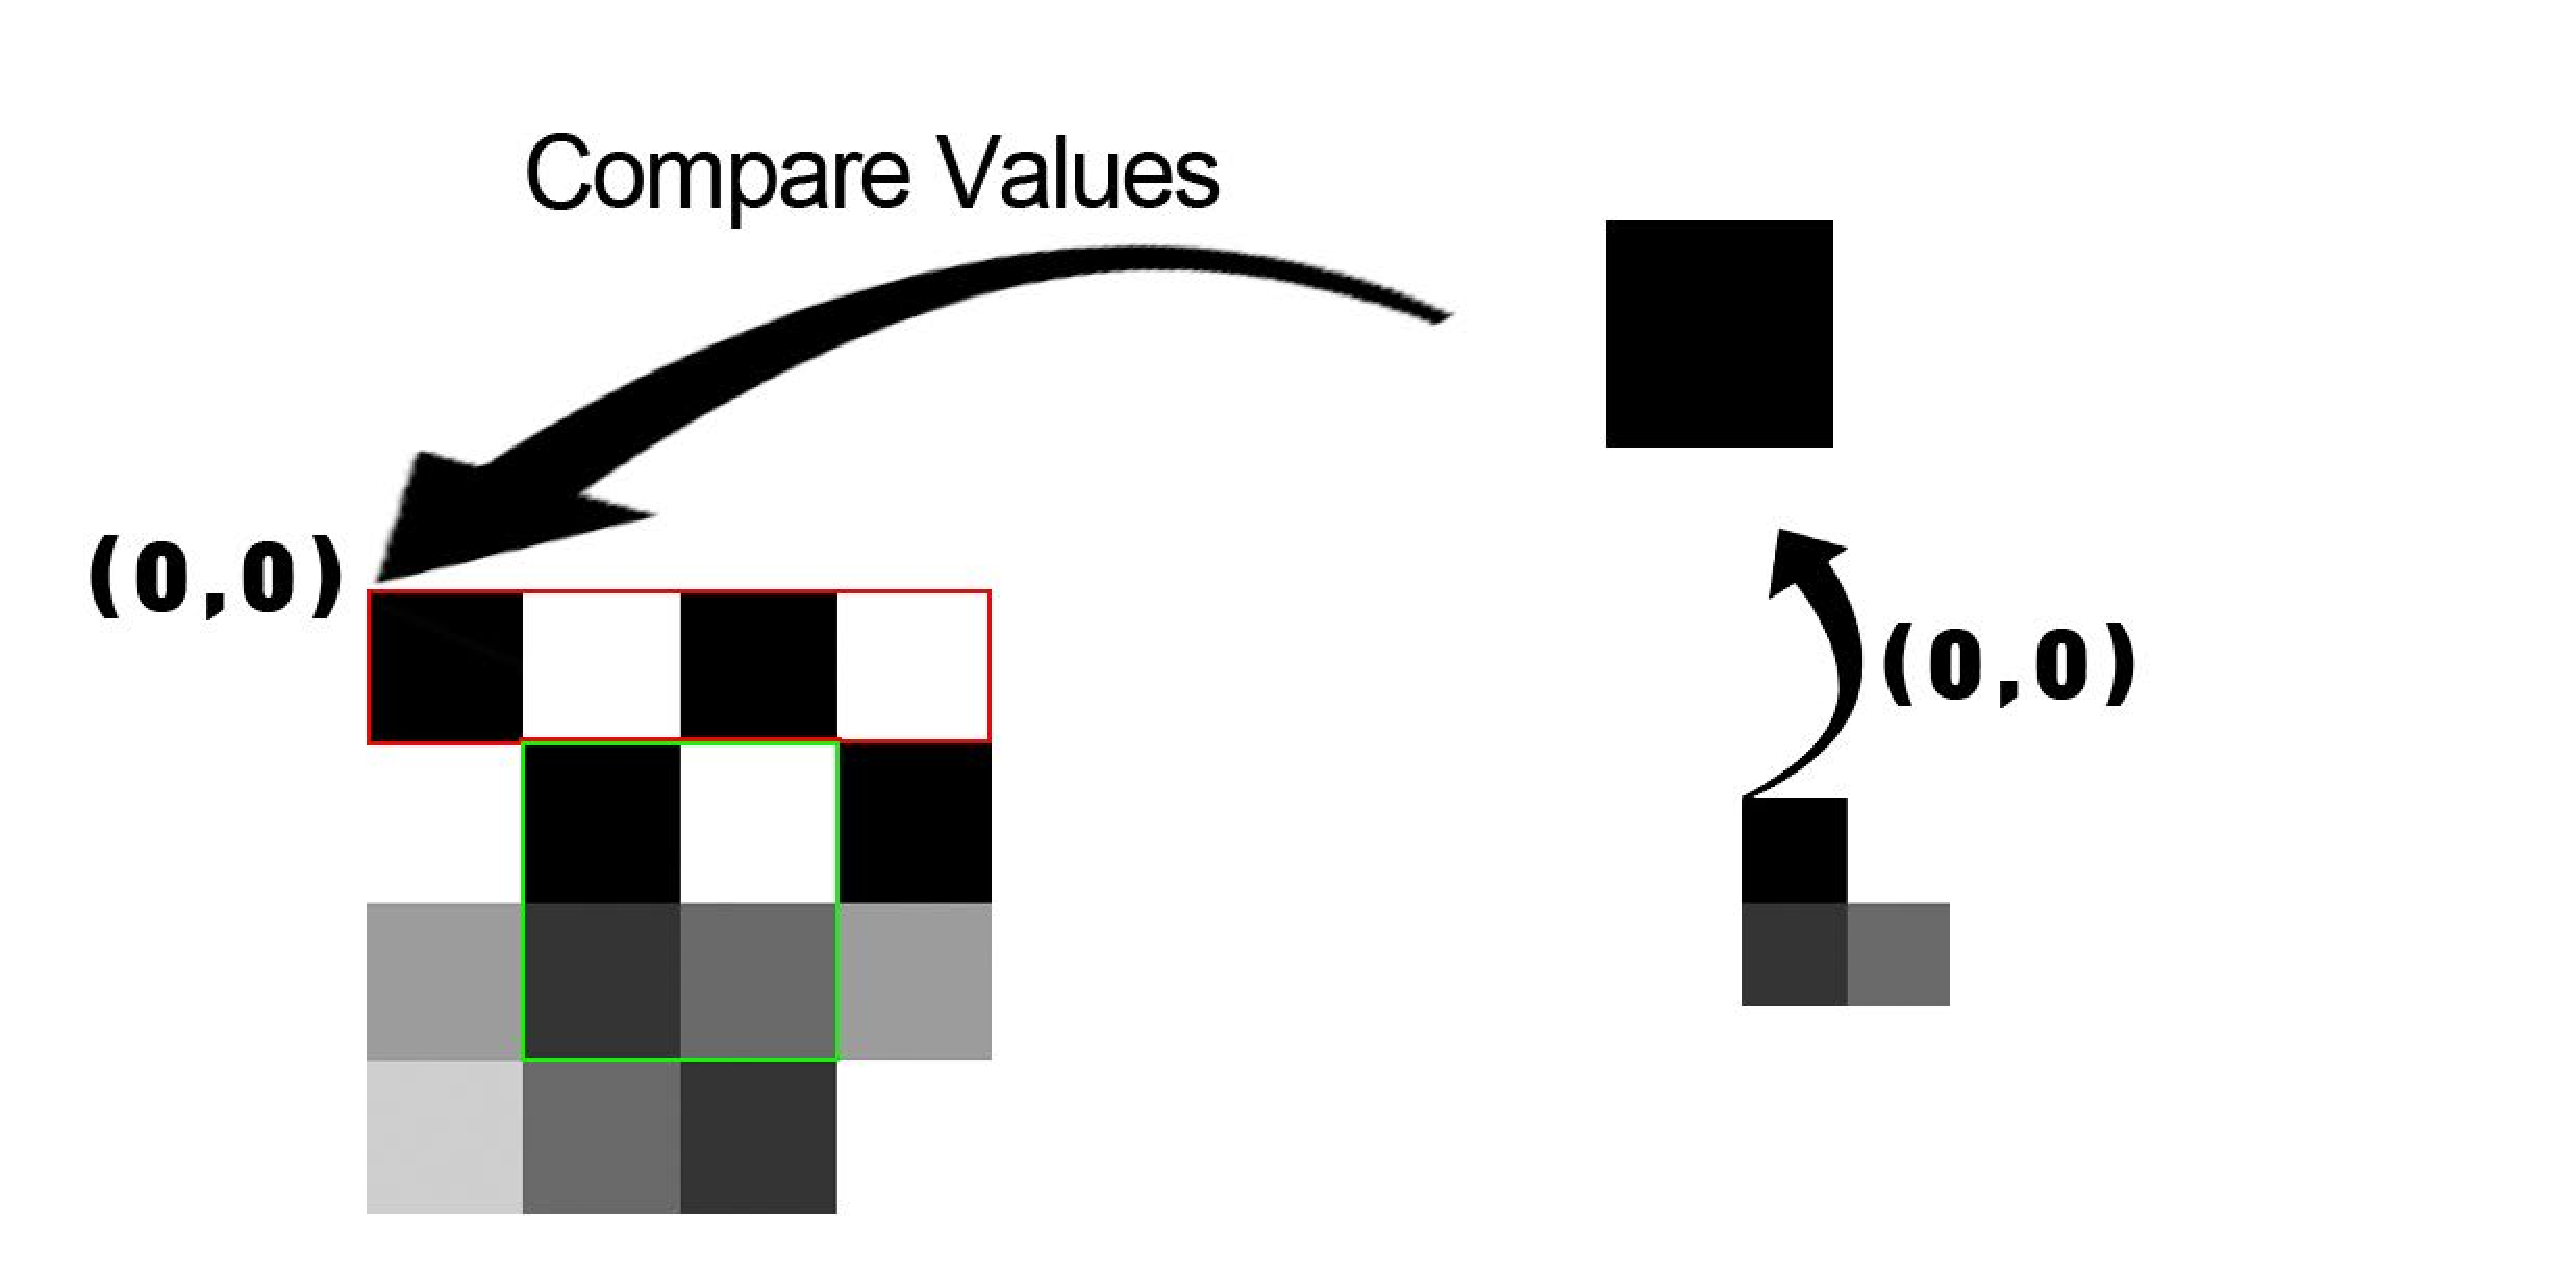
\includegraphics[scale=0.25]{images/Locate_Function.pdf}
        \caption{Figura representativa do funcionamento da ImageLocateSubImage()}
        \label{fig:locate}
    \end{figure}

    \par Após detetar um valor igual ao primeiro píxel da img2 na img1, é ainda comparado os restantes píxeis para 
        garantir que são iguais, podendo afirmar que img2 é, de facto, uma subimagem da img1. Para fazer essa 
        comparação é usado o seguinte excerto de código, onde i e j são, respetivamente, as coordenadas x e y da 
        img2, e são comparados os pixeis equivalentes. Para isso é adicionado ao i e j as coordenadas da img1, caso
        estejamos a localizar a img2 no ponto (x,y) que não seja (0,0) da img1.

    \begin{lstlisting}
        for(int j =0;j < img2->height;j++) {
            for(int i = 0;i < img2->width;i++) {
              if (ImageGetPixel(img1,x + i ,y + j) != ImageGetPixel(img2, i, j)) {
                return 0}
            }
        }
    \end{lstlisting}


    \newpage

    
\section{Image Blur}\label{sec:imageblur}
    \par A seguinte função visa a implementar um filtro de imagem de \textit{blur}, em que é aplicado um filtro da média de pixeis num dado retângulo de dimensão $(2dx + 1) \times (2dy + 1)$. \ Para tal, foram considerados dois algoritmos, detalhados nas subsecções seguintes.

\subsection{Algoritmo Melhorado}\label{subsec:blur1}
    \par Este algoritmo utiliza uma \href{https://en.wikipedia.org/wiki/Summed-area_table}{\textit{Summed-area table}}, definido por um \textit{array} bidimensional, com tamanho $width \times height$. \ Este pode ser dividido em duas partes: cálculo da soma das áreas em cada pixel e cálculo do \textit{blur} numa determinada área.

\subsubsection{Summed-area table}
    \par O seguinte método implementa uma forma de, em um dado ponto $(x,y)$, obter a soma de todos os valores dos pixeis desde $(0,0)$ a esse mesmo ponto. \ Da forma em que foi implementado, apenas é feita a média dos valores na atribuição na própria imagem, que resulta em o \textit{array} ser do tipo inteiro.

    \par A forma geral para a implementação deste algoritmo é:

    \begin{lstlisting}
      integral[x][y] = ImageGetPixel(img, x, y) +
      integral[x - 1][y] +
      integral[x][y - 1] -
      integral[x - 1][y - 1];    
    \end{lstlisting}

    \par Com o seguinte bloco de código, está a ser atribuído às coordenadas $(x,y)$ do \textit{array} criado anteriormente a soma total dos valores dos pixeis.
    \par Esta fórmula é visualmente representada na \autoref{fig:summedAreaTable}.

    \begin{figure} [H]
        \centering
        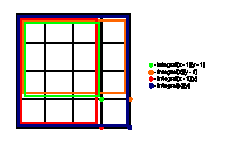
\includegraphics[scale=3]{images/sumareas.pdf}
        \caption{Figura ilustrativa do algoritmo \textit{Summed-area table}} 
        \label{fig:summedAreaTable}
    \end{figure}

    \newpage

    \par Ainda considerando o algoritmo anterior, Verifica-se um problema de \textit{assertion}, causado quando $x$ ou $y$ são 0. \ Para evitar esse problema, é atribuído inicialmente ao $(0,0)$ (já que a soma total nesse ponto é ele próprio) o seu próprio valor.

    \par De seguida, são preenchidas as linhas $x = 0$ e $y = 0$. \ Após isso, é possível preencher o resto do \textit{array} com a fórmula geral anteriormente apresentada.

\subsubsection{Média dos pixeis}
    \par O seguinte algoritmo é responsável por calcular a média dos pixeis numa determinada área, definida por um retângulo de dimensão $(2dx + 1) \times (2dy + 1)$. \ São usados os valores de soma obtidos na parte anterior.

    \par Inicialmente, são definidos o canto superior esquerdo e canto inferior direito, e verificar se o retângulo está dentro da imagem. \ Caso não esteja, é lhe atribuído o valor representante do extremo que está a ultrapassar.

    \par Finalmente, é calculada a média dos pixeis, com o seguinte bloco de código:

    \begin{lstlisting}
        (double)((integral[x2 - 1][y2 - 1] -
        integral[x1][y2 - 1] -
        integral[x2 - 1][y1] +
        integral[x1][y1])) /
        npixels + 0.5;
    \end{lstlisting}

    \par O valor de 0.5 é adicionado para que o valor seja arredondado corretamente, já que o valor é do tipo inteiro. \ Também é subtraído o valor de 1 a $x2$ e $y2$, de forma a que o valor seja o correto, já que o \textit{array} começa em $(0,0)$.

\subsubsection{Análise da Complexidade}
    \par Na \autoref{tab:complexidade}, é possível observar a complexidade de cada função, em termos de iterações de ciclos e de operações aritméticas das duas partes do algoritmo.

    \begin{table}[H]
        \centering
        \begin{tabular}{| p{23mm} | p{25mm} | p{30mm} | p{30mm} | p{38mm} |}
            \hline

            \textbf{Imagem} & \textbf{Fator de \textit{blur}} & \textbf{Iterações de 3.1.1.} & \textbf{Iterações de 3.1.2} & \textbf{Complexidade} \\ \hline

            original.pgm (300x300) & $7,7$ & $90000$ & $90000$ & $O((width \times height) \times 2)$ \\ \hline

            original.pgm (300x300) & $40,40$ & $90000$ & $90000$ & $O((width \times height) \times 2)$ \\ \hline

            original.pgm (300x300) & $200,200$ & $90000$ & $90000$ & $O((width \times height) \times 2)$ \\ \hline

            airfield.pgm (1600x1200) & $40,40$ & $1920000$ & $1920000$ & $O((width \times height) \times 2)$ \\ \hline

            airfield.pgm (1600x1200) & $200,200$ & $1920000$ & $1920000$ & $O((width \times height) \times 2)$ \\ \hline

            ireland.pgm (640x480) & $40,40$ & $307200$ & $307200$ & $O((width \times height) \times 2)$ \\ \hline
        \end{tabular}
        \caption{Tabela com a complexidade das funções}
        \label{tab:complexidade}
    \end{table}

    \newpage

    \par Como é possível observar na \autoref{tab:complexidade}, a complexidade das funções é $O((width \times height) \times 2)$, já que o número de iterações é igual ao número de pixeis da imagem. \ A complexidade das operações aritméticas é linear, já que o número de operações é igual ao número de pixeis da imagem. \ Isto resulta em:

    \begin{itemize}
        \item \textbf{Best case} - A imagem ser pequena;
        \item \textbf{Average case} - Não existe um caso médio, já que a complexidade é sempre a mesma;
        \item \textbf{Worst case} - A imagem ser grande.
    \end{itemize}

\subsection{Algoritmo Básico}\label{subsec:blur2}
    \par Como o nome indica, este algoritmo é mais básico, que acaba por ser menos eficiente que o anterior. \ Este algoritmo baseia-se em ir de pixel a pixel da imagem, e de pixel a pixel da área definida pelo retângulo de dimensão $(2dx + 1) \times (2dy + 1)$, verificar se esse pixel se encontra dentro da imagem e calcular a média dos pixeis nessa área dependendo do resultado.

\subsubsection{Análise da complexidade}
    \par Na \autoref{tab:complexidade2} é apresentado a complexidade geral do algoritmo, em termos de iterações de ciclos.

    \begin{table}[H]
        \centering
        \begin{tabular}{| p{23mm} | p{25mm} | p{30mm} | p{38mm} |}
            \hline

            \textbf{Imagem} & \textbf{Fator de \textit{blur}} & \textbf{Iterações de 3.2.1.} & \textbf{Complexidade} \\ \hline

            original.pgm (300x300) & $7,7$ & $20250000$ & $O((2dx + 1) \times (2dy + 1) \times w \times h)$ \\ \hline

            original.pgm (300x300) & $40,40$ & $590490000$ & $O((2dx + 1) \times (2dy + 1) \times w \times h)$ \\ \hline

            original.pgm (300x300) & $200,200$ & $14472090000$ & $O((2dx + 1) \times (2dy + 1) \times w \times h)$ \\ \hline

            airfield.pgm (1600x1200) & $40,40$ & $12597120000$ & $O((2dx + 1) \times (2dy + 1) \times w \times h)$ \\ \hline

            airfield.pgm (1600x1200) & $200,200$ & $308737920000$ & $O((2dx + 1) \times (2dy + 1) \times w \times h)$ \\ \hline

            ireland.pgm (640x480) & $40,40$ & $2015539200$ & $O((2dx + 1) \times (2dy + 1) \times w \times h)$ \\ \hline
        \end{tabular}
        \caption{Tabela com a complexidade das funções}
        \label{tab:complexidade2}
    \end{table}

    \par Como é possível observar na \autoref{tab:complexidade2}, a complexidade das funções é $O((2dx + 1) \times (2dy + 1) \times w \times h)$, já que o número de iterações está dependente desta vez não só pelo tamanho da imagem, mas também pelo tamanho do fator do \textit{blur}. \ Isto resulta em obter como:

    \begin{itemize}
        \item \textbf{Best case} - A imagem ser pequena e o fator de blur ser pequeno;
        \item \textbf{Average case} - Um \textit{balance} entre o tamanho da imagem e o fator de blur;
        \item \textbf{Worst case} - A imagem ser grande e o fator de blur ser grande.
    \end{itemize}


    \newpage

    \section{Conclusão}
    \par Concluindo, neste projeto foi possível implementar várias funções de manipulação de imagem, de grau de dificuldade variável, e a análise de complexidade de duas delas. 
    \par Foi possível observar que, após a análise de vários algoritmos, a mesma função com o mesmo objetivo pode ter mudanças bastante significantes em termos de tempo de execução em vários cenários.

    \par Este trabalho foi realizado por:
        \begin{itemize}
            \item \authorjp - 50\%
            \item \authorrg - 50\% 
        \end{itemize}

    \begin{flushright}
        \today
    \end{flushright}


\end{document}